\documentclass[t]{beamer}
\usetheme{Copenhagen}
\setbeamertemplate{headline}{} % remove toc from headers
\beamertemplatenavigationsymbolsempty

\usepackage{amsmath, tikz, bm, tkz-euclide,pgfplots}
\pgfplotsset{compat = 1.16}
\usetkzobj{all}

\title{Complex Numbers}
\author{}
\date{}

\AtBeginSection[]
{
  \begin{frame}
    \frametitle{Objectives}
    \tableofcontents[currentsection]
  \end{frame}
}

\begin{document}

\begin{frame} 
\maketitle
\end{frame}

\section{Write square roots of negative numbers as imaginary numbers}

\begin{frame}{Background}
Imaginary numbers arose from trying to solve equations such as 
\[x^2 = -1\] \pause

If we take the square root of both sides, we get 
\[ x = \sqrt{-1} \]	\pause

We define the imaginary unit $i$ to be that value:
\[ i = \sqrt{-1} \]
\end{frame}

\begin{frame}{Writing Square Roots of Negative Numbers}
When writing square roots of negative values as imaginary numbers, we can factor out \[\sqrt{-1}\] from the expression \newline\\

{\color{blue}\textbf{as long as what remains is the square root of a positive number.}}
\begin{align*}
\onslide<2->{\sqrt{-25} &= \sqrt{-1} \cdot \sqrt{25} }\\[6pt] 
\onslide<3->{&= i \cdot 5} \\[6pt]	\pause
\onslide<4->{&= 5i}
\end{align*}
\end{frame}

\begin{frame}{Example 1}
Write each as an imaginary number.	\newline\\
(a) \quad $\sqrt{-36}$
\begin{align*}
\onslide<2->{\sqrt{-36} &= \sqrt{-1} \cdot \sqrt{36}} \\[6pt]
\onslide<3->{&= i \cdot 6} \\[6pt]
\onslide<4->{&= 6i}
\end{align*}
\end{frame}

\begin{frame}{Example 1}
(b) \quad $\sqrt{-100}$
\begin{align*}
\onslide<2->{\sqrt{-100} &= \sqrt{-1} \cdot \sqrt{100}} \\[6pt]
\onslide<3->{&= i \cdot 10} \\[6pt]
\onslide<4->{&= 10i}
\end{align*}
\end{frame}

\begin{frame}{Example 1}
(c) \quad $\sqrt{-8}$
\begin{align*}
\onslide<2->{\sqrt{-8} &= \sqrt{-1} \cdot \sqrt{8}} \\[6pt]
\onslide<3->{&= i \cdot 2\sqrt{2}} \\[6pt]
\onslide<4->{&= 2i\sqrt{2}}
\end{align*}
\end{frame}

\section{Add and subtract complex numbers}

\begin{frame}{Complex Numbers}
A \alert{complex number} is a number written in the form
\[ a + bi \]
where $a$ (the \alert{real part}) and $b$ (the \alert{imaginary part}) are real numbers.
\end{frame}

\begin{frame}{Adding and Subtracting Complex Numbers}
Complex numbers can be added and subtracted much like combining like terms in Algebra 1.	\newline\\	\pause

The real parts are added (or subtracted) together, as are the imaginary parts.	\newline\\	\pause

Answers are then typically written in $a + bi$ form.
\end{frame}

\begin{frame}{Example 2}
Simplify each. \newline\\ 
(a) \quad $(3 + 2i) + (-1 + 8i)$
\begin{align*}
\onslide<2->{(3+2i)+(-1+8i)&= (3+(-1))+(2i+8i)} \\[6pt]
\onslide<3->{&= 2 + 10i}
\end{align*}
\end{frame}

\begin{frame}{Example 2}
(b) \quad $(-5-i) + (2+4i)$
\begin{align*}
\onslide<2->{(-5-i) + (2+4i)&= (-5+2)+(-i+4i)} \\[6pt]
\onslide<3->{&= -3+3i}
\end{align*}
\end{frame}

\begin{frame}{Example 2}
(c) \quad $(7-9i) - (3+5i)$
\begin{align*}
\onslide<2->{(7-9i) - (3+5i)&= 7-9i-3-5i} \\[6pt]
\onslide<3->{&= 4-14i}
\end{align*}
\end{frame}

\begin{frame}{Example 2}
(d) \quad $(-1+2i) - (-8+10i)$
\begin{align*}
\onslide<2->{(-1+2i) - (-8+10i)&= -1+2i+8-10i} \\[6pt]
\onslide<3->{&= 7-8i}
\end{align*}
\end{frame}

\section{Multiply complex numbers}

\begin{frame}{Multiplying Complex Numbers}
Complex numbers can be multiplied in the same manner that binomials are multiplied in Algebra 1, such as $(x+3)(x-8)$.	\newline\\	\pause

However, since $i = \sqrt{-1}$, if we \alert{square both sides} we get
\[ i^2 = -1 \]	\pause

So when multiplying complex numbers, you will substitute a $-1$ whenever you see an $i^2$.
\end{frame}

\begin{frame}{Example 3}
Multiply each.	\newline\\
(a) \quad $(2+3i)(5+6i)$	\newline\\
\onslide<2->{
\begin{center}
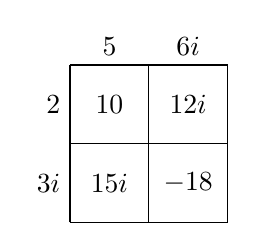
\begin{tikzpicture}
\draw[black] (0,0) grid (2,2);
\node at (0,1.5) [left] {$2$};
\node at (0,0.5) [left] {$3i$};
\node at (0.5,2) [above] {$5$};
\node at (1.5,2) [above] {$6i$};
\onslide<3->{\node at (0.5,1.5) {$10$};}
\onslide<4->{\node at (1.5,1.5) {$12i$};}
\onslide<5->{\node at (0.5,0.5) {$15i$};}
\onslide<6->{\node at (1.5,0.5) {$18i^2$};}
\onslide<7->{\node[fill=white, scale=2.5] at (1.5,0.5) {};}
\onslide<8->{\node at (1.5,0.5) {$-18$};}
\end{tikzpicture}
\end{center}
}
\onslide<9->{\[-8 + 27i\]}
\end{frame}

\begin{frame}{Example 3}
(b) \quad $(-1+i)(4-3i)$	\newline\\
\onslide<2->{
\begin{center}
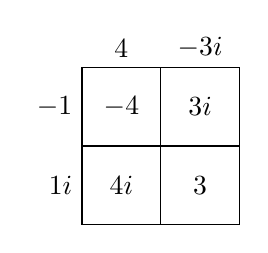
\begin{tikzpicture}
\draw[black] (0,0) grid (2,2);
\node at (0,1.5) [left] {$-1$};
\node at (0,0.5) [left] {$1i$};
\node at (0.5,2) [above] {$4$};
\node at (1.5,2) [above] {$-3i$};
\onslide<3->{\node at (0.5,1.5) {$-4$};}
\onslide<4->{\node at (1.5,1.5) {$3i$};}
\onslide<5->{\node at (0.5,0.5) {$4i$};}
\onslide<6->{\node at (1.5,0.5) {$-3i^2$};}
\onslide<7->{\node[fill=white, scale=3] at (1.5,0.5) {};}
\onslide<8->{\node at (1.5,0.5) {$3$};}
\end{tikzpicture}
\end{center}
}
\onslide<9->{\[-1 + 7i\]}
\end{frame}

\begin{frame}{Example 3}
(c) \quad $(7-7i)(7+7i)$	\newline\\
\onslide<2->{
\begin{center}
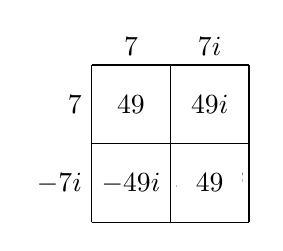
\begin{tikzpicture}
\draw[black] (0,0) grid (2,2);
\node at (0,1.5) [left] {$7$};
\node at (0,0.5) [left] {$-7i$};
\node at (0.5,2) [above] {$7$};
\node at (1.5,2) [above] {$7i$};
\onslide<3->{\node at (0.5,1.5) {$49$};}
\onslide<4->{\node at (1.5,1.5) {$49i$};}
\onslide<5->{\node at (0.5,0.5) {$-49i$};}
\onslide<6->{\node at (1.5,0.5) {$-49i^2$};}
\onslide<7->{\node[fill=white, scale=3.55] at (1.5,0.5) {};}
\onslide<8->{\node at (1.5,0.5) {$49$};}
\end{tikzpicture}
\end{center}
}
\onslide<9->{\[98\]}
\end{frame}

\section{Divide complex numbers}

\begin{frame}{Dividing Complex Numbers}
Dividing complex numbers presents a bit of a challenge. \newline\\	\pause

The reason is that the denominator will have a square root, which is a big no-no in math:	\pause

\[\frac{3-i}{2+i} = \frac{3-\sqrt{-1}}{2+\sqrt{-1}} \]	\pause

To remedy this, we need to find the \alert{conjugate} of the {\color{blue}\textbf{denominator}}.
\end{frame}

\begin{frame}{Complex Conjugates}
The \alert{conjugate} of a complex number 
\[ a + bi \] 
is
\[a - bi \] 
and vice versa
\end{frame}

\begin{frame}{Conjugate Examples}
\begin{center}
\begin{tabular}{cc}
\textbf{Number} & \textbf{Conjugate} \\ \hline
\onslide<2->{$7+2i$} & \onslide<3->{$7-2i$} \\[6pt]
\onslide<4->{$-3+i$} & \onslide<5->{$-3-i$} \\[6pt]
\onslide<6->{$5-4i$} & \onslide<7->{$5+4i$} \\[6pt]
\end{tabular}	\newline\\
\end{center}
\onslide<8->{When you multiply complex conjugates, you will always get a real number, like in Example 3c.}	\newline\\
\onslide<9->{So, to divide complex numbers, multiply both numerator and denominator by the {\color{blue}\textbf{conjugate of the denominator}}.}
\end{frame}

\begin{frame}{Example 4}
Divide $\dfrac{3-i}{2+i}$. Write your answer in $a+bi$ form.	\newline\\
\onslide<2->{The conjugate of $2+i$ is $2-i$}
\begin{align*}
\onslide<3->{\frac{3-i}{2+i}}\onslide<4->{\left(\frac{2-i}{2-i}\right)&} \\[10pt]
\onslide<5->{&=\frac{5-5i}{5}} \\[10pt]
\onslide<6->{&=1-i}
\end{align*}
\end{frame}

\end{document}